% !TEX root = ../../技术文档.tex
\section{NPU仿真验证}

本节整理NPU计算、缓冲、DMA和控制接口的模块及子系统仿真结果。
波形以ModelSim Wave窗口截图展示，数值结果采用对应测试台与整数参考模型的比较记录。
各用例分别注明阵列规模、量化通路和存储模型，按其实际组件配置统计结果。50\,MHz、$M=2$、单量化通路的头像应用整机验证另见附录\ref{sec:box-system-validation}。
截图来源、测试记录和文件校验值保存于\path{docs/verification/npu/report_waveforms_3523d03/}。

表\ref{tbl:npu-simulation-results}汇总代表性数值用例与向量算子回归结果。
前三项是空间层回归中的单个用例；后两项分别统计两种量化配置下的向量算子集合。

\begin{reporttable}
\small
\begin{longtable}{@{}p{0.19\linewidth}p{0.46\linewidth}r@{}}
\caption{NPU代表性数值验证结果}\label{tbl:npu-simulation-results}\\
\toprule
测试对象 & 测试配置与比较范围 & 匹配字节数 \\
\midrule
\endfirsthead
\caption[]{NPU代表性数值验证结果（续）}\\
\toprule
测试对象 & 测试配置与比较范围 & 匹配字节数 \\
\midrule
\endhead
\bottomrule
\endfoot
DW16 & 17通道，$4\times19$输出位置，S16，Q4时分量化 & 2584 \\
MaxPool & 64通道，$7\times41$输出位置，7行写回 & 18368 \\
Resize & 3通道，$40\times38$输出位置，40行写回 & 4560 \\
向量算子回归 & 共享八通道量化器、片上存储原语及本地存储模型，14例 & 150092 \\
向量算子回归 & Q4时分量化、片上存储原语及本地存储模型，9例 & 149212 \\
\end{longtable}
\end{reporttable}

\subsection{计算正确性}\label{sec:npu-compute-validation}

普通卷积阵列采用$M=16$的组件配置，观察$K$向量接收、乘加提交和本地累加器更新，波形如图\ref{fig:npu-dense-validation}所示。
\texttt{in\_k}与\texttt{retire\_k}分别标记输入和提交的归约索引，\texttt{accepted}与\texttt{retired}记录对应事件数，\texttt{pending}记录在途向量数。
第0路累加器\texttt{acc\_flat[31:0]}随有效提交更新，测试台同时检查其余通路及异常输入。
阵列回归包含9个正常用例和12个错误用例，统计223次接收、219次提交和4次清空，结束时在途计数为0。

\begin{figure}[!htbp]
\centering
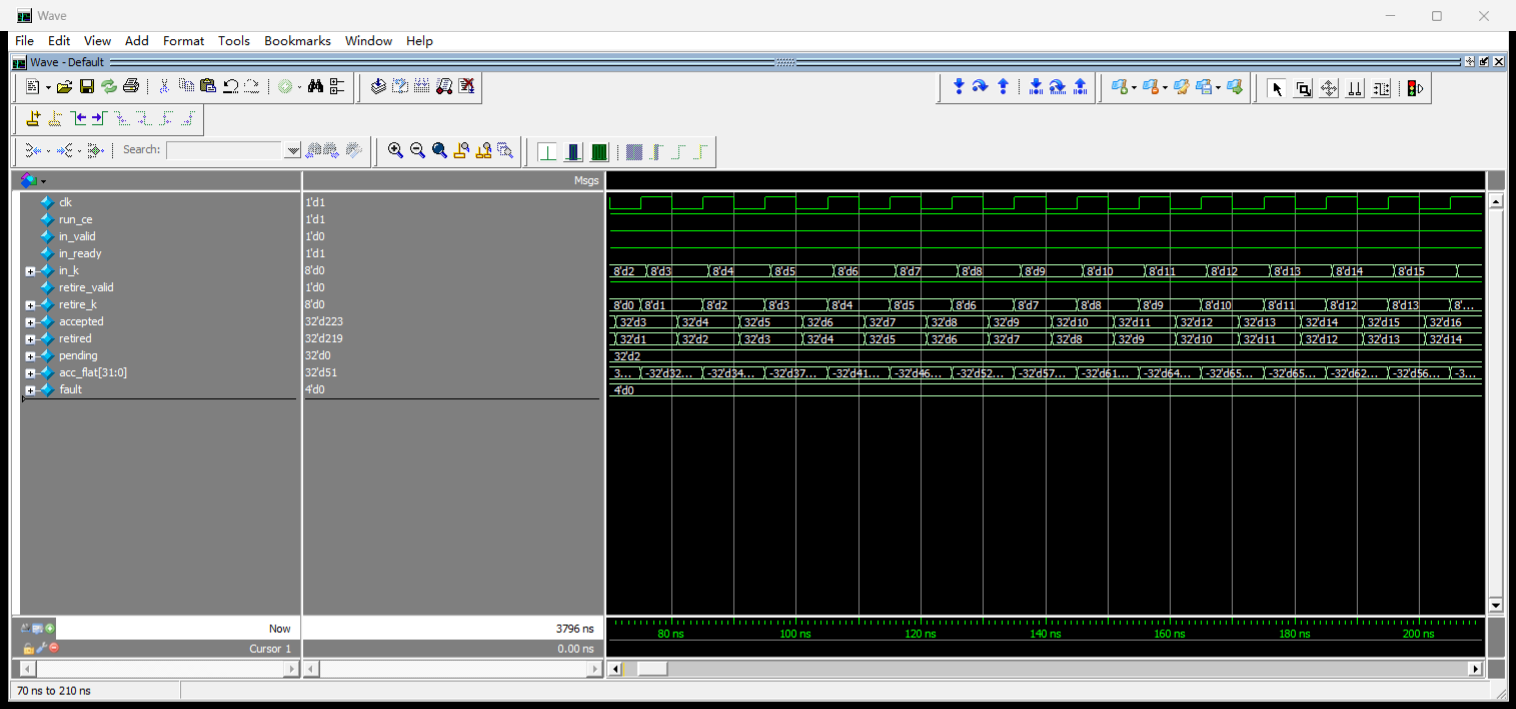
\includegraphics[width=\linewidth,height=0.52\textheight,keepaspectratio]{../figure/npu-simulation/dense-accumulate.png}
\caption{普通卷积阵列的输入、提交与累加波形（$M=16$组件配置）}\label{fig:npu-dense-validation}
\end{figure}

DW16用例采用17个输入、输出通道，覆盖一个完整16通道组和一个尾通道，输出尺寸为$4\times19$。
图\ref{fig:npu-dw-validation}记录层控制状态、运算计数和完成信号。
两个通道组分别遍历76个空间位置和9个核采样点，共产生1368个MAC向量；按该用例的Q4时分量化配置，统计304个量化组和4行写回。
测试台对$17\times4\times19\times2=2584$\,B的S16输出逐字节比较，结果与整数参考一致。

\begin{figure}[!htbp]
\centering
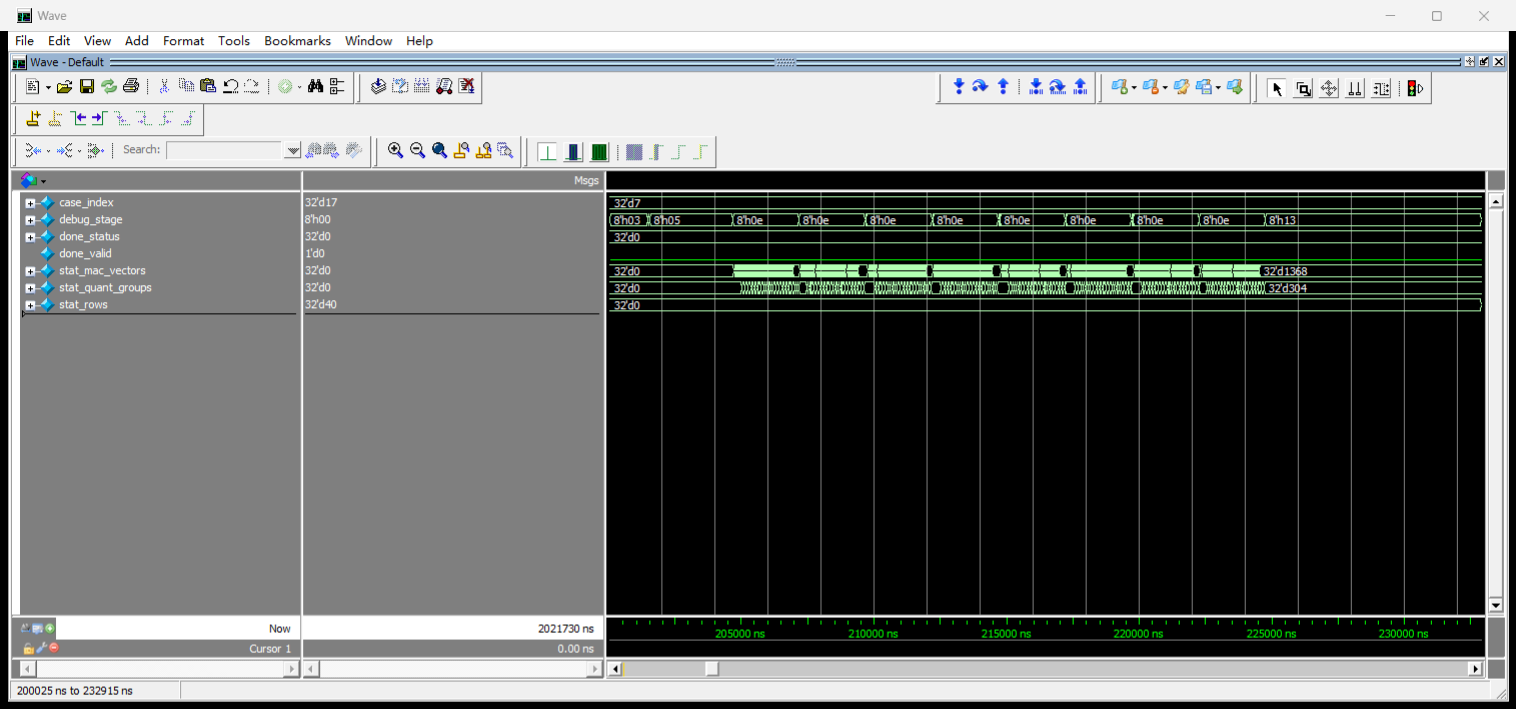
\includegraphics[width=\linewidth,height=0.52\textheight,keepaspectratio]{../figure/npu-simulation/dw16-tail-channel.png}
\caption{DW16尾通道用例的层级计数与完成波形}\label{fig:npu-dw-validation}
\end{figure}

定点后处理单元的数值验证采用八条物理量化通路，检查Bias相加、整数系数乘法、右移、最近偶数舍入及目标类型限幅。
输入接收与输出交付同时受共同推进条件和\texttt{run\_ce}控制；暂停或输出背压期间，待交付数据和标签保持稳定。
图\ref{fig:npu-quant-validation}上窗展示混合样本的输入与输出，下窗展示第0路有符号重定标和U8限幅：舍入结果为$-64$时，输出值为0。
该单元回归核对105321个有效通道算术样本，并覆盖256种通道掩码、输出保持及清空恢复。
图中的周期和流水延迟按八通道单元配置记录，正文中的单、双通路配置采用相同整数规则。

\begin{figure}[!htbp]
\centering
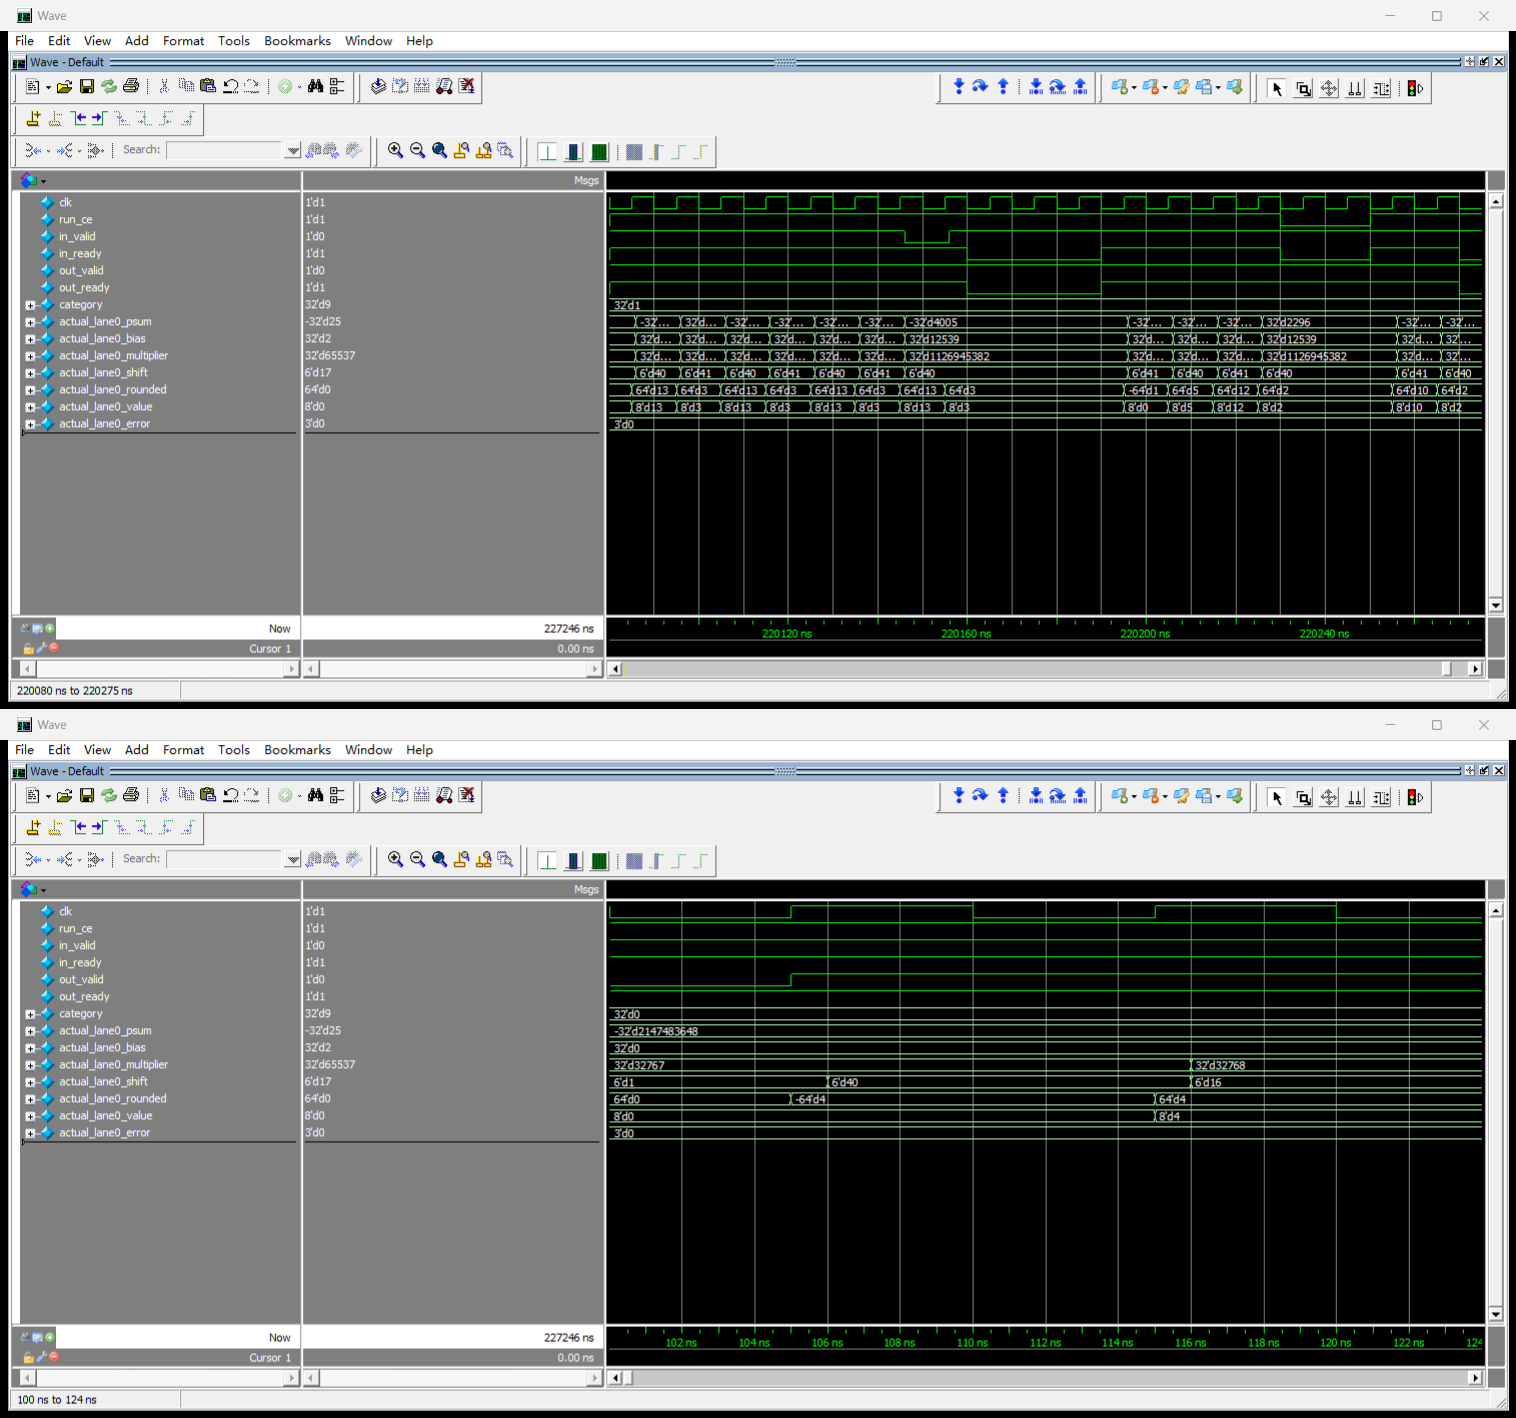
\includegraphics[width=\linewidth,height=0.52\textheight,keepaspectratio]{../figure/npu-simulation/quantization.png}
\caption{定点后处理的重定标与U8限幅波形（八通道单元配置）}\label{fig:npu-quant-validation}
\end{figure}

\subsection{分块计算}\label{sec:npu-tiling-validation}

输入缓冲验证分别检查驻留行复用和卷积窗口供数，波形如图\ref{fig:npu-input-validation}所示。
上窗采用$C_{\rm in}=64$的驻留命中用例，输入行已保存在片上；行装载状态更新用时两拍，期间外部读请求和读返回保持无效。
下窗采用独立的窗口生成用例，\texttt{roi\_req\_a}给出ROI读取请求，\texttt{a\_write\_valid}与\texttt{a\_write\_index}标记依次写入的A向量。
两个窗口分别沿用各自用例的时间轴。测试台依据输入张量、窗口坐标及补边规则检查返回数据与写入索引。

\begin{figure}[!htbp]
\centering
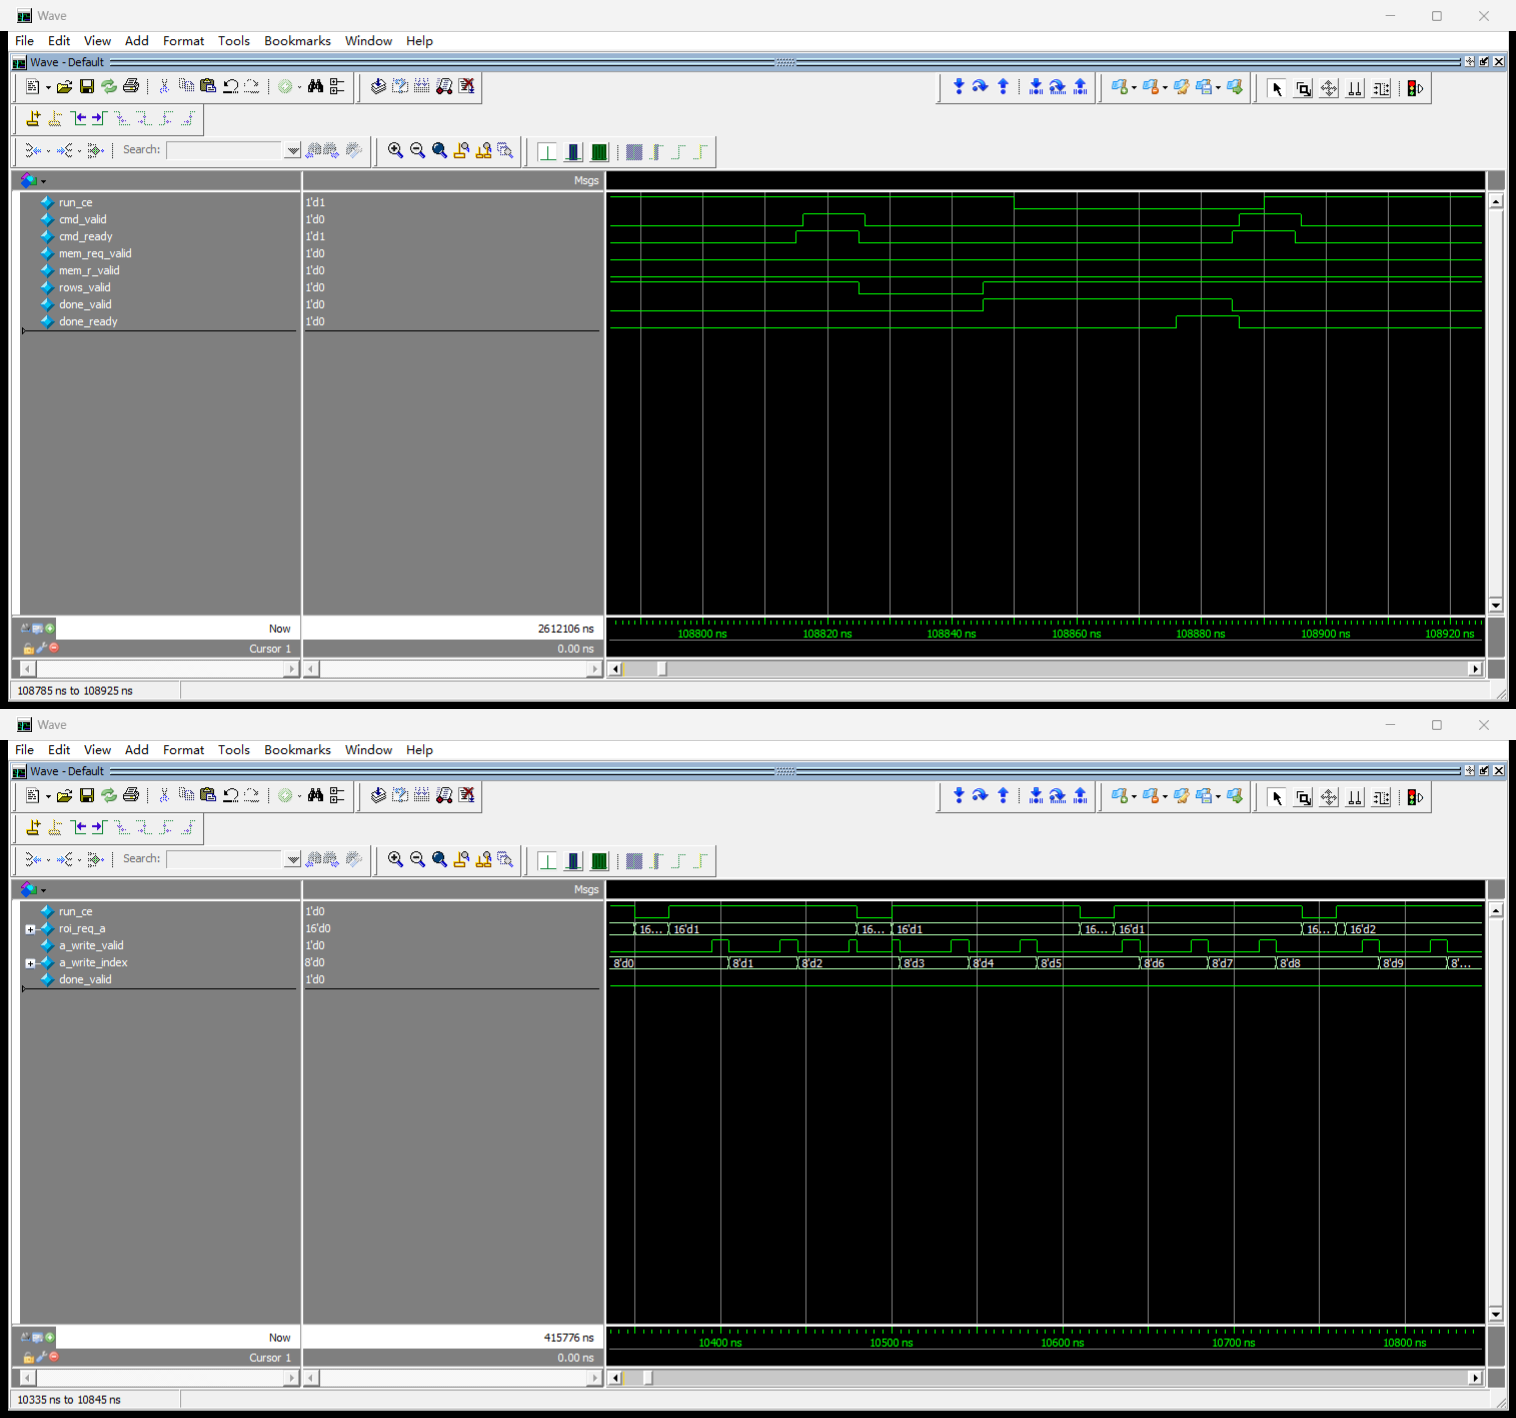
\includegraphics[width=\linewidth,height=0.52\textheight,keepaspectratio]{../figure/npu-simulation/input-gather.png}
\caption{输入行驻留复用与卷积窗口供数波形}\label{fig:npu-input-validation}
\end{figure}

输出尾块用例采用16空间位置、16输出通道的缓存组合配置，其中7个空间位置和9个输出通道有效。
每个位置的量化结果按8个通道和1个尾通道写入，字节使能限定实际更新范围。
图\ref{fig:npu-output-validation}上窗显示512位\texttt{o\_valid}有效字节位图及量化组计数，下窗显示本地读请求和读响应。
位图中每一位对应一个字节的有效状态；测试台按有效位置比较输出，并以预置哨兵检查相邻无效区域。
同一缓存组合回归共核对3840个O数据字和720个A/B/P/O保护区数据字，读回结果均一致。

\begin{figure}[!htbp]
\centering
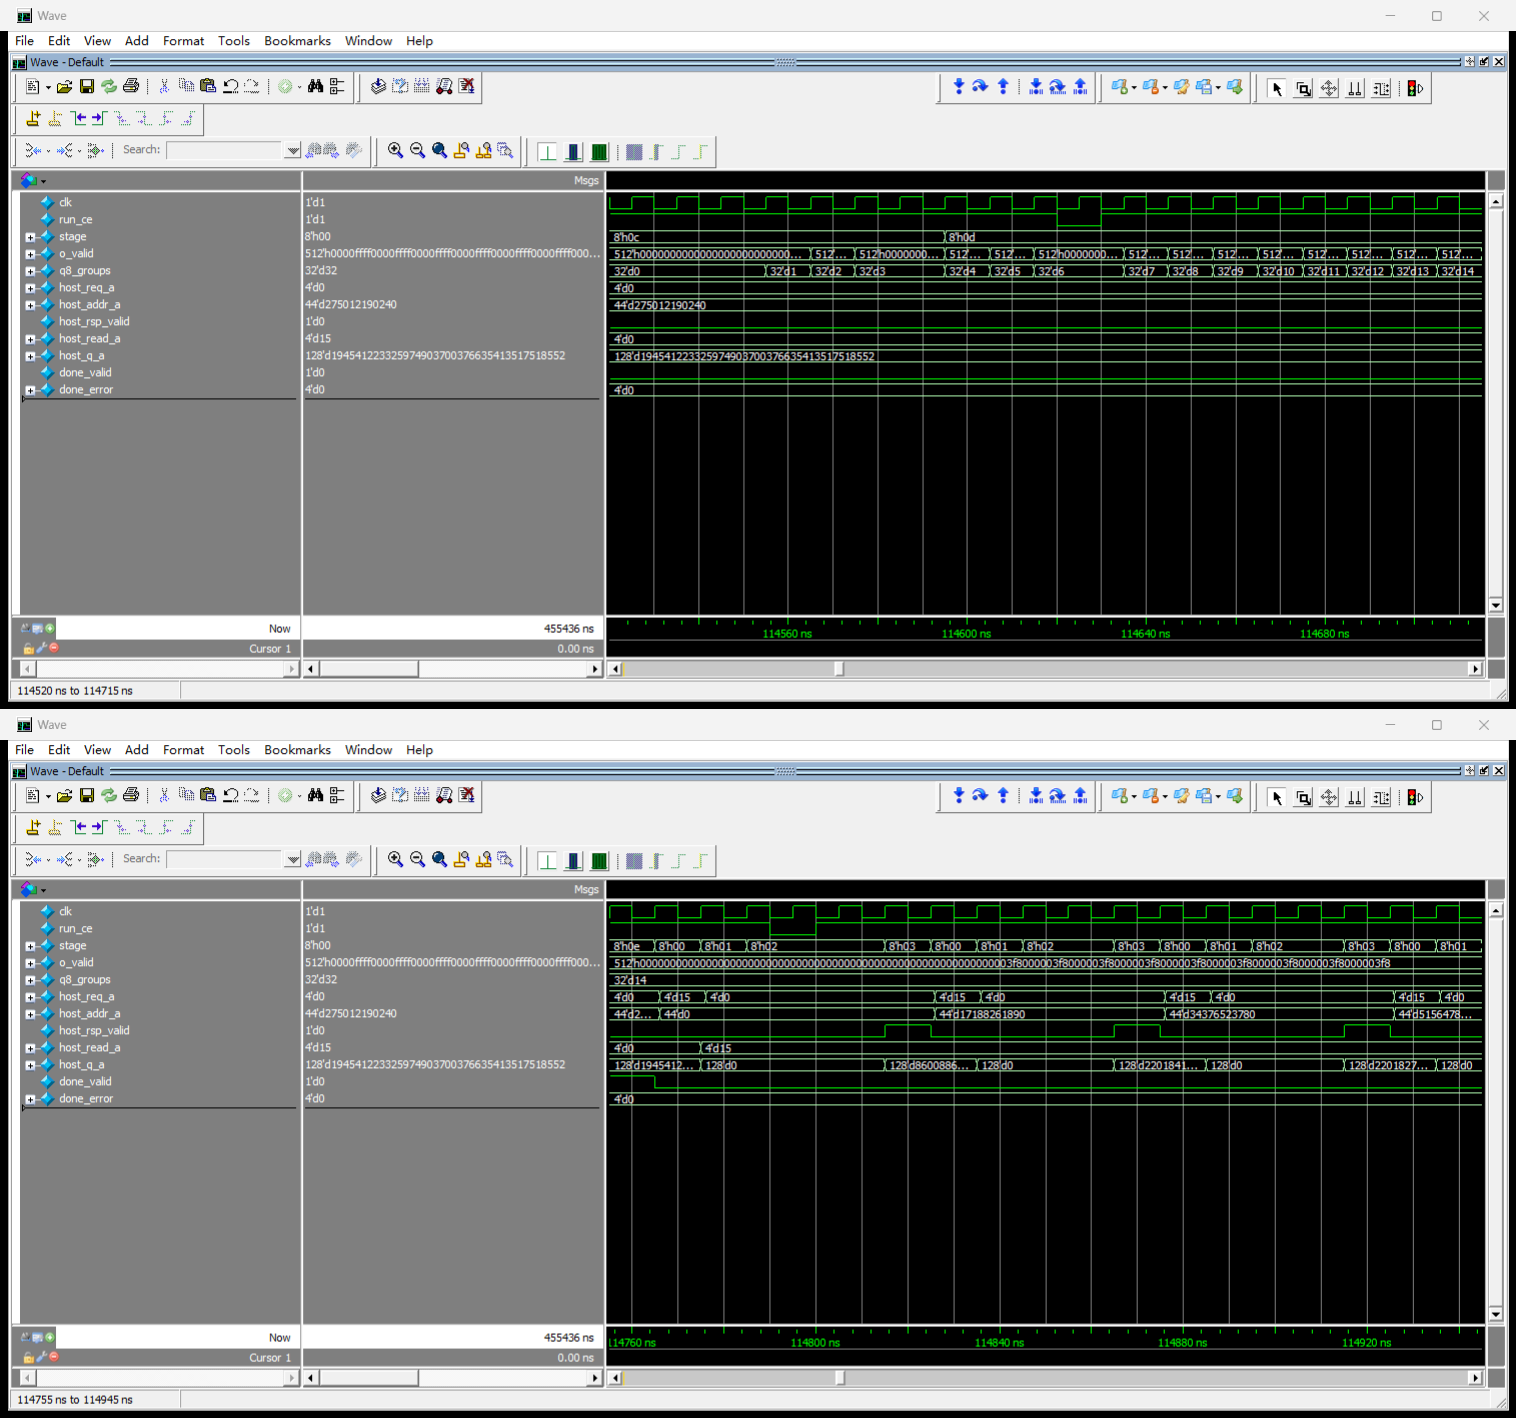
\includegraphics[width=\linewidth,height=0.52\textheight,keepaspectratio]{../figure/npu-simulation/output-mask.png}
\caption{输出尾块的有效字节位图与本地读回波形}\label{fig:npu-output-validation}
\end{figure}

\subsection{DMA传输}\label{sec:npu-dma-validation}

块传输验证采用独立读写桥，本地域运行于100\,MHz，DDR用户接口域运行于125\,MHz，连接HMIC控制器和两颗x16 DDR3器件模型。
测试台发出写入与读回命令，在读数据和完成接口施加背压，并逐字节检查返回值。
图\ref{fig:npu-dma-validation}截取用例17至20，展示地址接收、写数据末拍、读返回末拍和本地完成握手。
\texttt{done\_valid}保持至\texttt{done\_ready}允许接收，完成状态随记录一并交付。

\begin{figure}[!htbp]
\centering
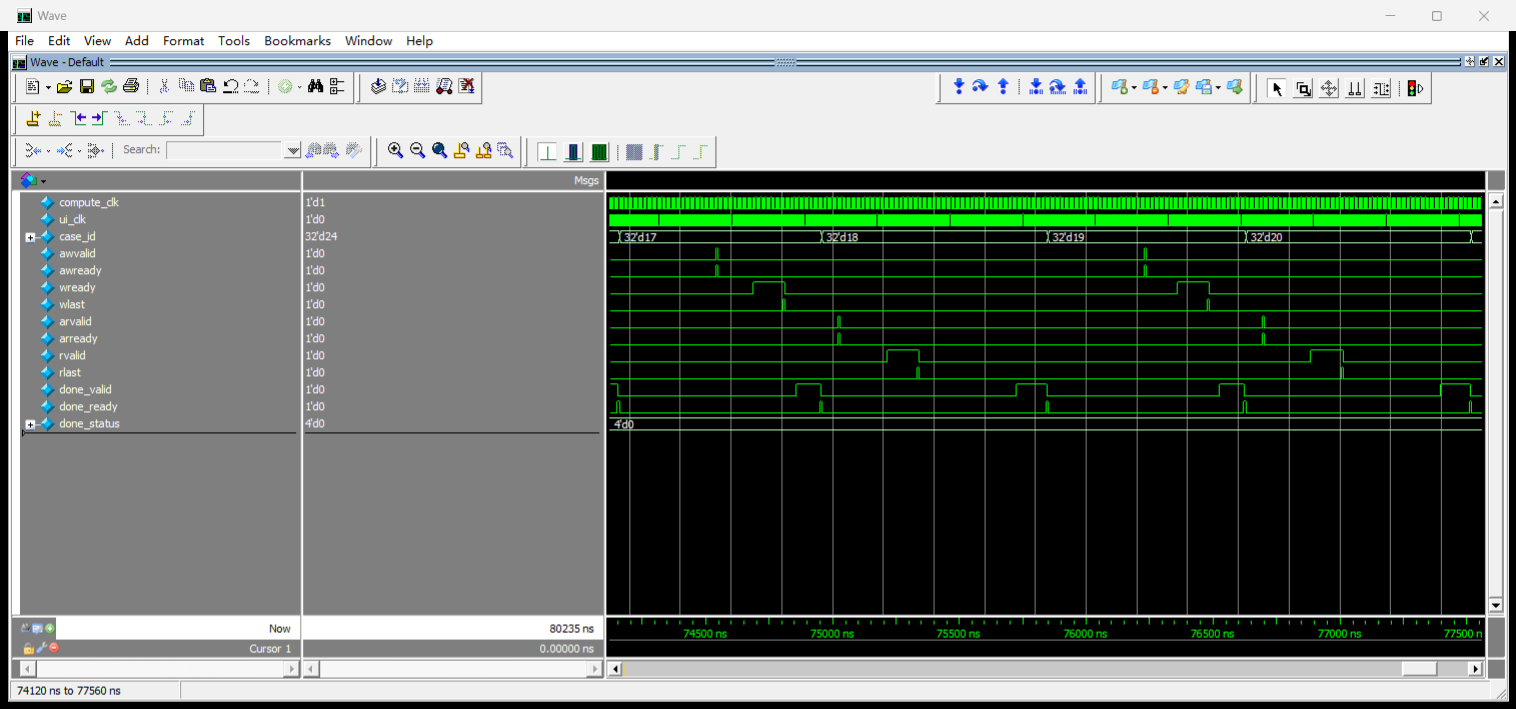
\includegraphics[width=\linewidth,height=0.52\textheight,keepaspectratio]{../figure/npu-simulation/dma-completion.png}
\caption{独立读写桥的跨时钟域传输与完成握手波形}\label{fig:npu-dma-validation}
\end{figure}

该器件模型用例执行12次写入和12次读取，原生写拍与读返回拍均为101拍，3232次字节比较全部匹配。
覆盖的突发长度为1、2、8、15、16拍，同时检查全字节写、交替字节掩码和4\,KiB边界两侧访问。
测试台完成259次本地读数据保持检查、240次完成记录保持检查和1746次事务所有权保持检查。
上述结果的统计范围为独立桥同一端口的功能读写与完成顺序。
器件模型记录保留267条连接或端口警告，以及84条初始化和写校准运行时警告；功能数据比较与器件时序检查分别记录。

\subsection{任务控制}\label{sec:npu-control-validation}

单算子MMIO验证检查参数锁存、启动接收、完成等待、任务身份核对和故障响应。
图\ref{fig:npu-mmio-validation}上窗展示层核提出完成时外部事务尚在处理的情况：\texttt{done\_valid}有效后，\texttt{retired}为0，\texttt{done\_ready}保持为0；
外部事务结束后，接口接收完成记录。
下窗展示故障状态的置位及复位清除。配套用例分别注入错误任务标签和会话标识变化，检查接口对任务身份的判定。
该接口回归共464项检查通过，覆盖AXI4-Lite写地址与写数据独立到达、背压、身份匹配ACK及完成发布条件。

\begin{figure}[!htbp]
\centering
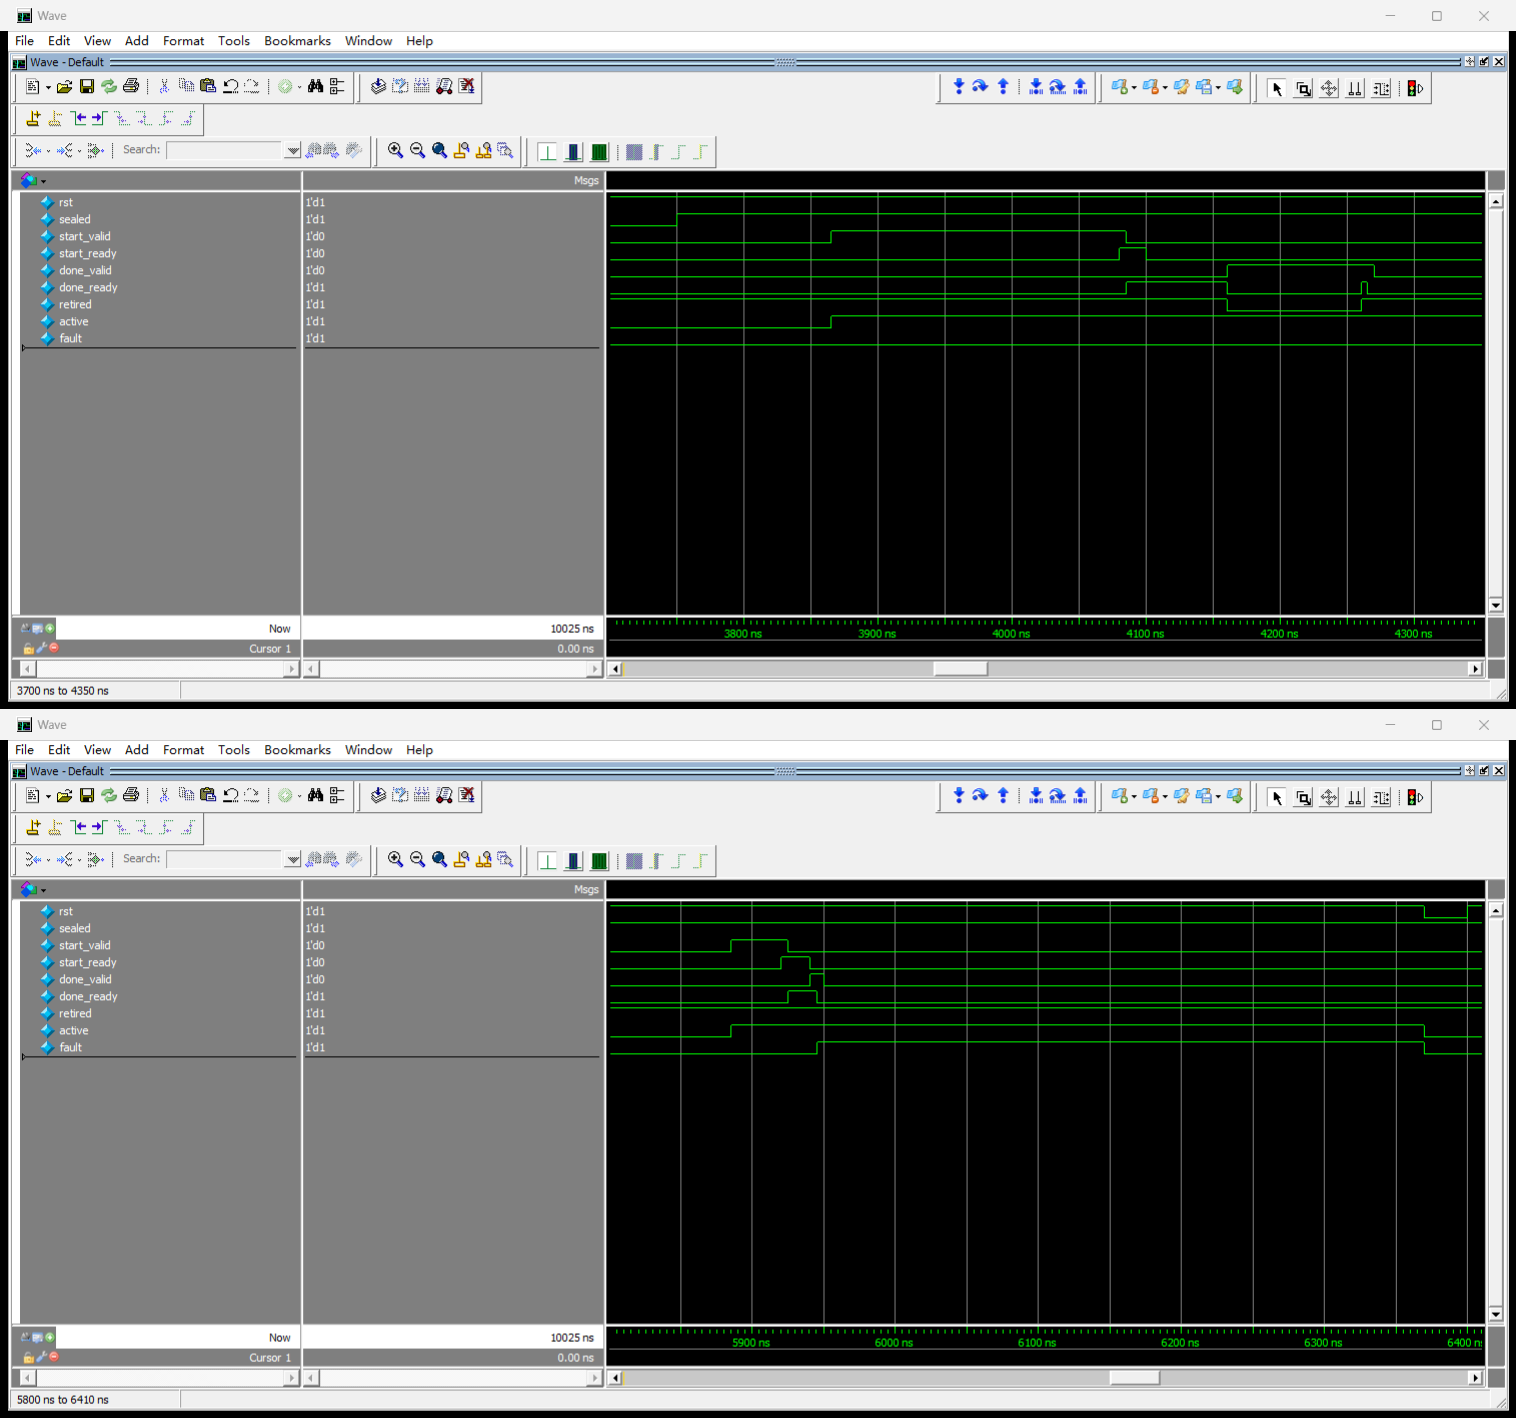
\includegraphics[width=\linewidth,height=0.52\textheight,keepaspectratio]{../figure/npu-simulation/layer-mmio.png}
\caption{单算子接口的完成等待与故障响应波形}\label{fig:npu-mmio-validation}
\end{figure}

输入FIFO验证以参考实现与载荷有效位适配实现逐拍比较公开端口，覆盖清空、复位、暂停和重新装载。
图\ref{fig:npu-fifo-validation}中，清空后占用计数与\texttt{payload\_live}均归零，公开输出\texttt{od\_dut}与参考输出\texttt{od\_ref}一致。
私有存储体保留的字节由有效位隔离；重新装载后，两种实现恢复相同的计数和输出序列。
完整回归记录3202888项检查通过，检查范围包含公开数据、计数、时钟使能、未知载荷及清空复位行为。

\begin{figure}[!htbp]
\centering
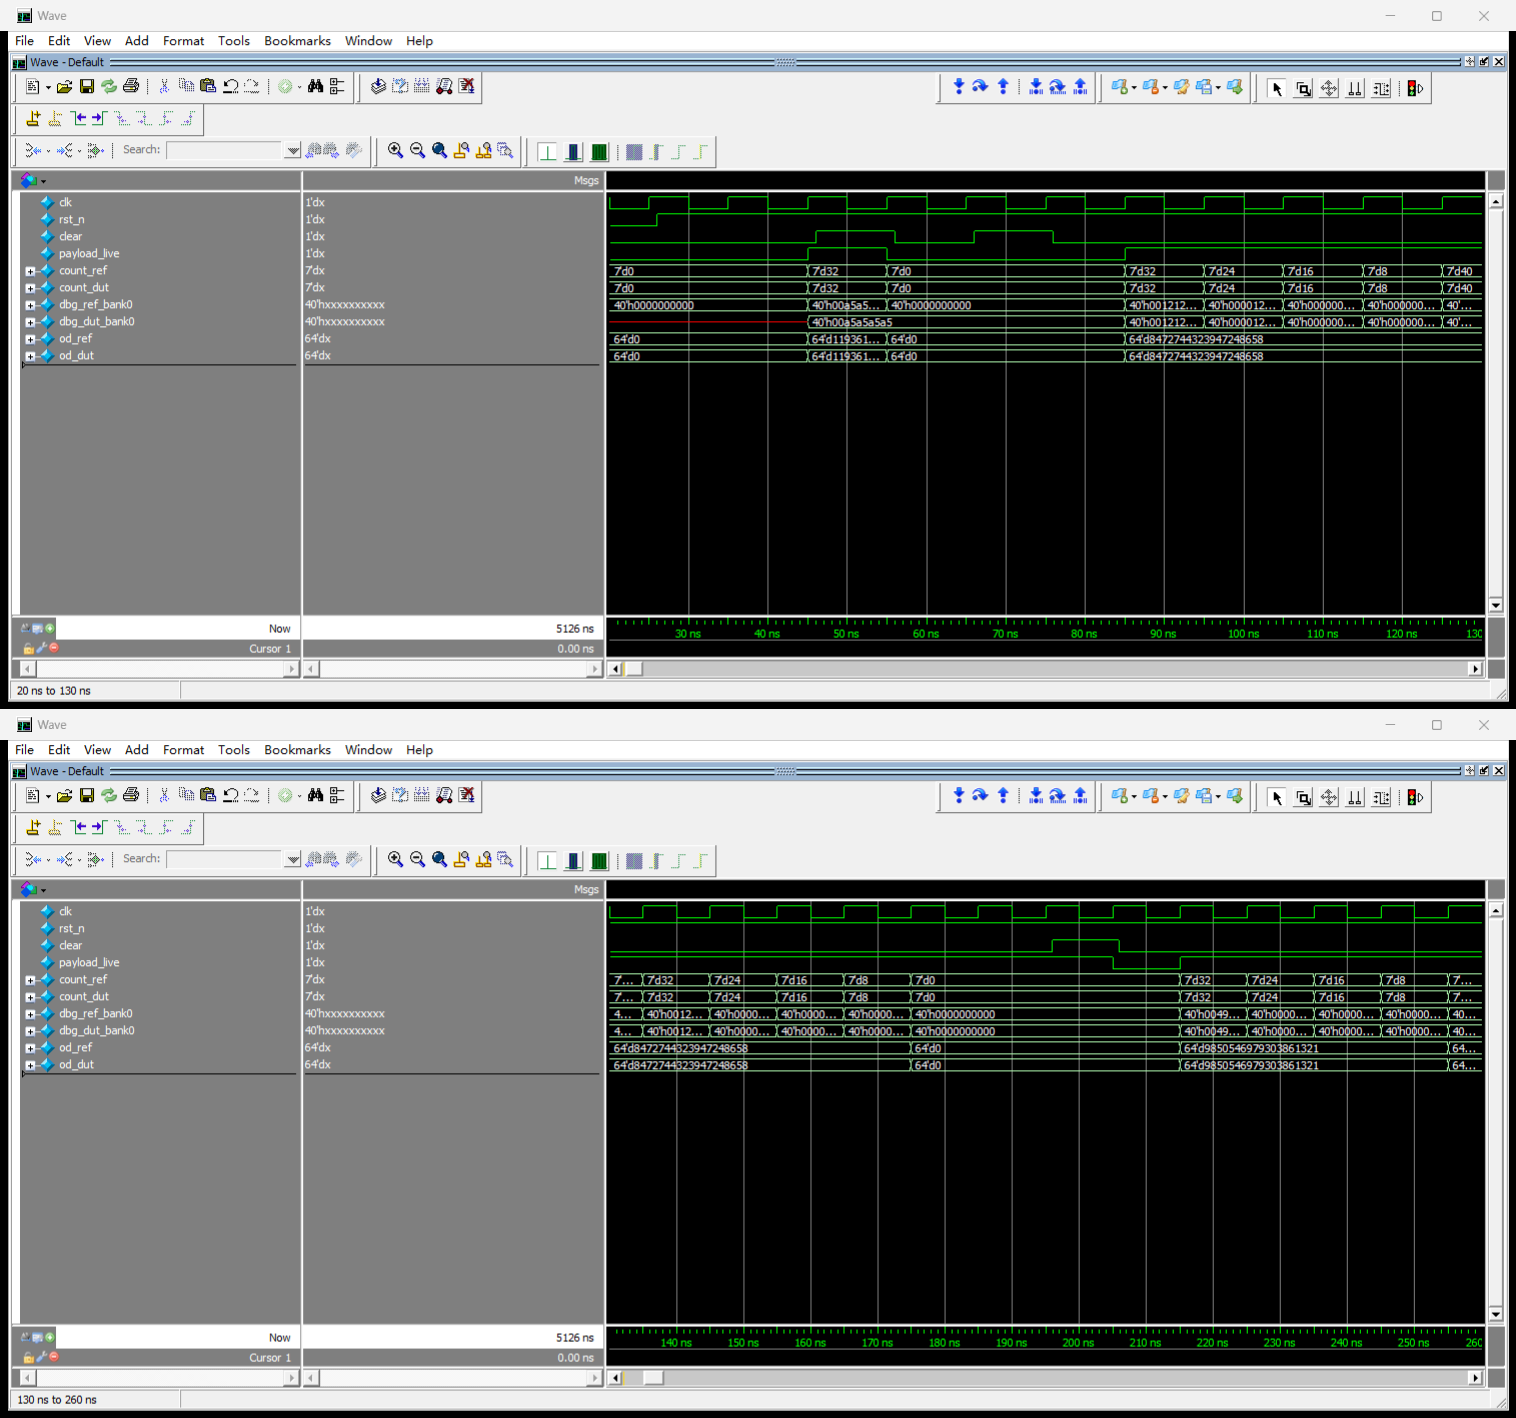
\includegraphics[width=\linewidth,height=0.52\textheight,keepaspectratio]{../figure/npu-simulation/fifo-clear.png}
\caption{输入FIFO清空、载荷隔离与重新装载波形}\label{fig:npu-fifo-validation}
\end{figure}

\subsection{辅助算子}\label{sec:npu-aux-validation}

Add、Sigmoid、Transpose和Reshape共用向量存储端口，测试台通过本地存储模型提供输入并核对输出。
八通道量化配置的回归覆盖14个用例、150092\,B；Q4时分量化配置的回归覆盖9个用例、149212\,B，分别与独立整数参考逐字节一致。
图\ref{fig:npu-vector-validation}取自Q4配置，显示Add和Sigmoid第一组量化处理的状态边界。
状态值\texttt{0x0C}、\texttt{0x0E}、\texttt{0x0F}和\texttt{0x10}依次对应量化准备、请求、等待结果和概率表读取请求。
Add在量化等待后返回准备状态，处理下一组元素；Sigmoid在量化等待后发出概率表读取请求。
状态的含义依据该用例的RTL定义解释，数据比较采用测试台的独立记录。

\begin{figure}[!htbp]
\centering
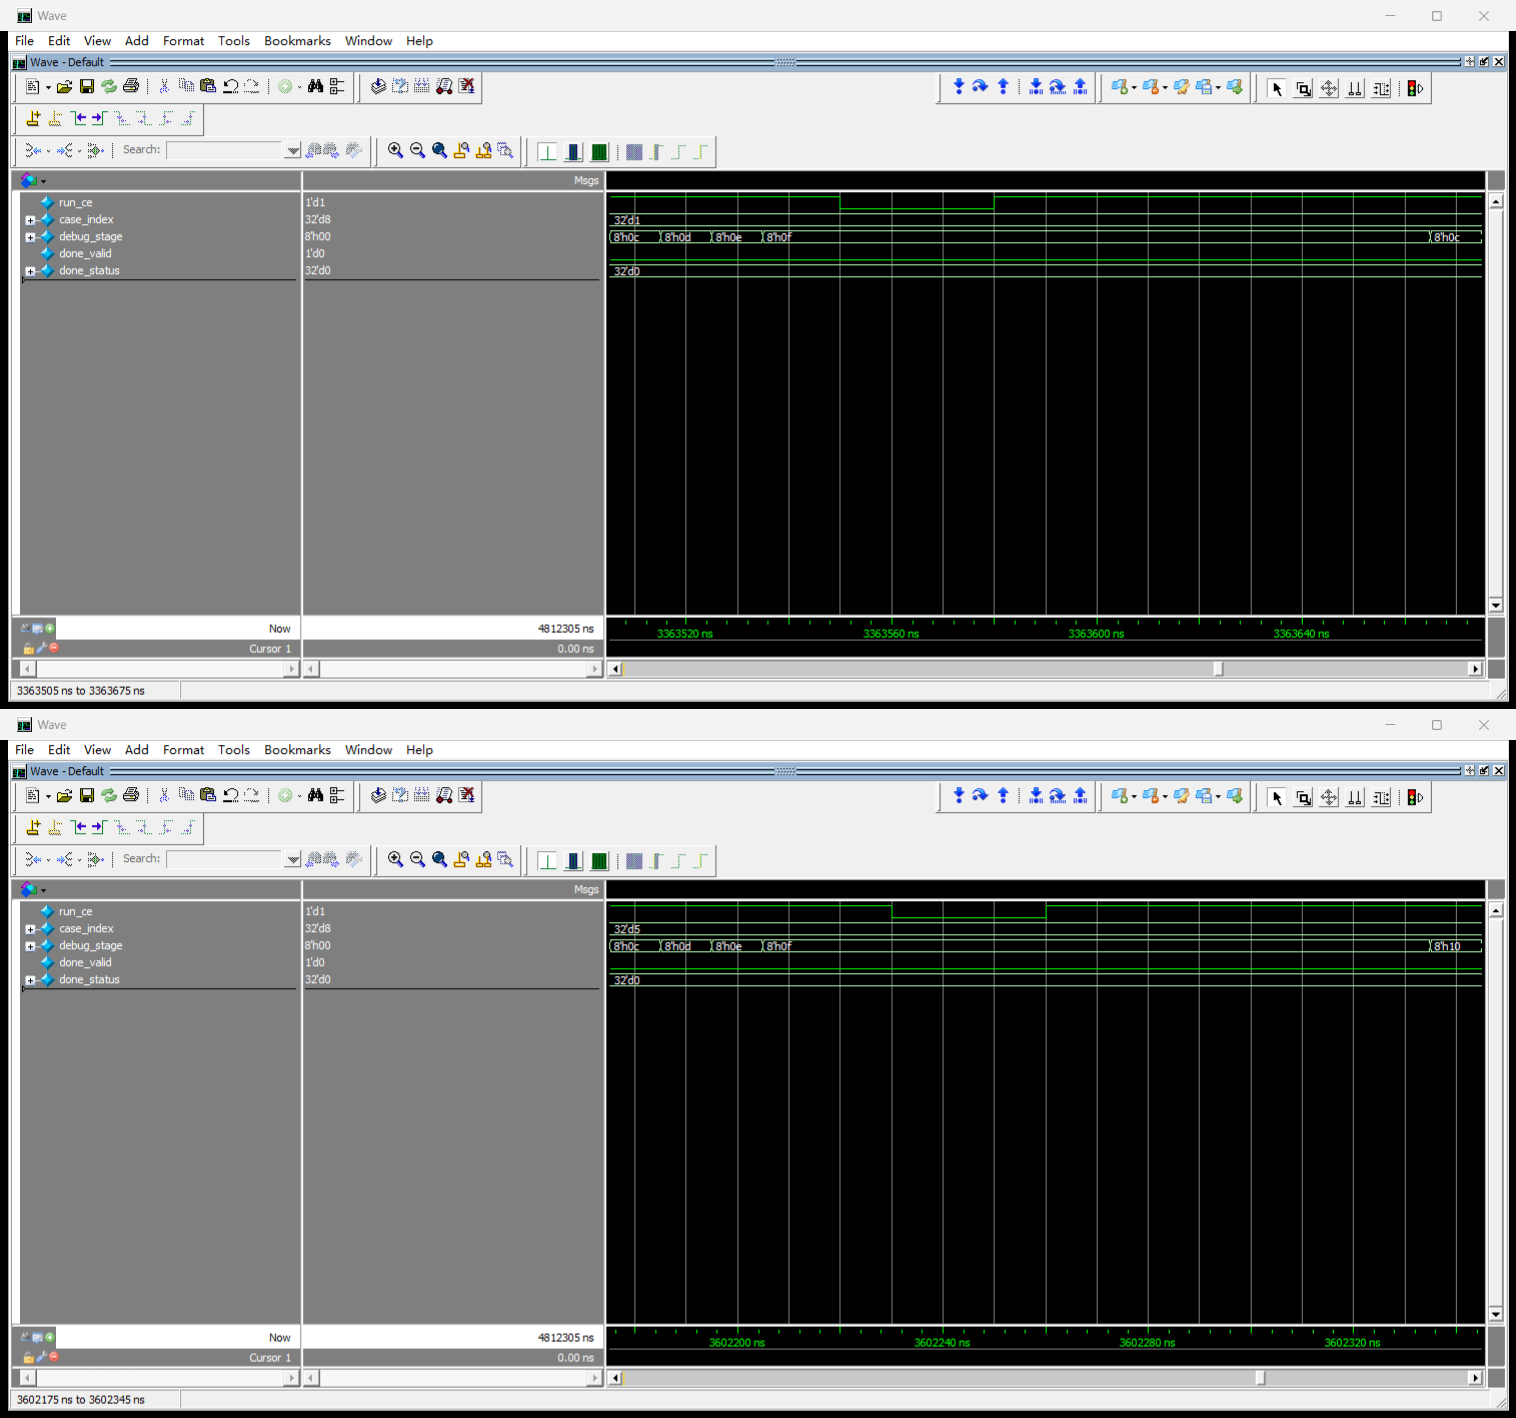
\includegraphics[width=\linewidth,height=0.52\textheight,keepaspectratio]{../figure/npu-simulation/vector-quantization.png}
\caption{Add与Sigmoid的量化处理状态波形（Q4时分配置）}\label{fig:npu-vector-validation}
\end{figure}

Transpose用例按目标维序搬运$4\times1\times17$个I16元素，136\,B输出全部匹配。
Reshape用例保持6400个I16元素的顺序，12800\,B输出全部匹配。
相关回归同时检查读写背压、元素边界和目的缓冲区相邻区域，确保地址变换与有效字节写入一致。

MaxPool与Resize采用空间层和块DMA联合仿真，桥端使用字节存储模型，计算及片上缓冲使用相应RTL和器件原语。
图\ref{fig:npu-pool-resize-validation}分别截取两个用例的末行写回与完成过程。
MaxPool产生7行、18368\,B输出，Resize产生40行、4560\,B输出，均与独立整数参考一致。
两个用例的MAC向量计数和量化组计数保持为0，\texttt{stat\_rows}在末行写回后分别达到7和40，随后\texttt{done\_valid}置位。

\begin{figure}[!htbp]
\centering
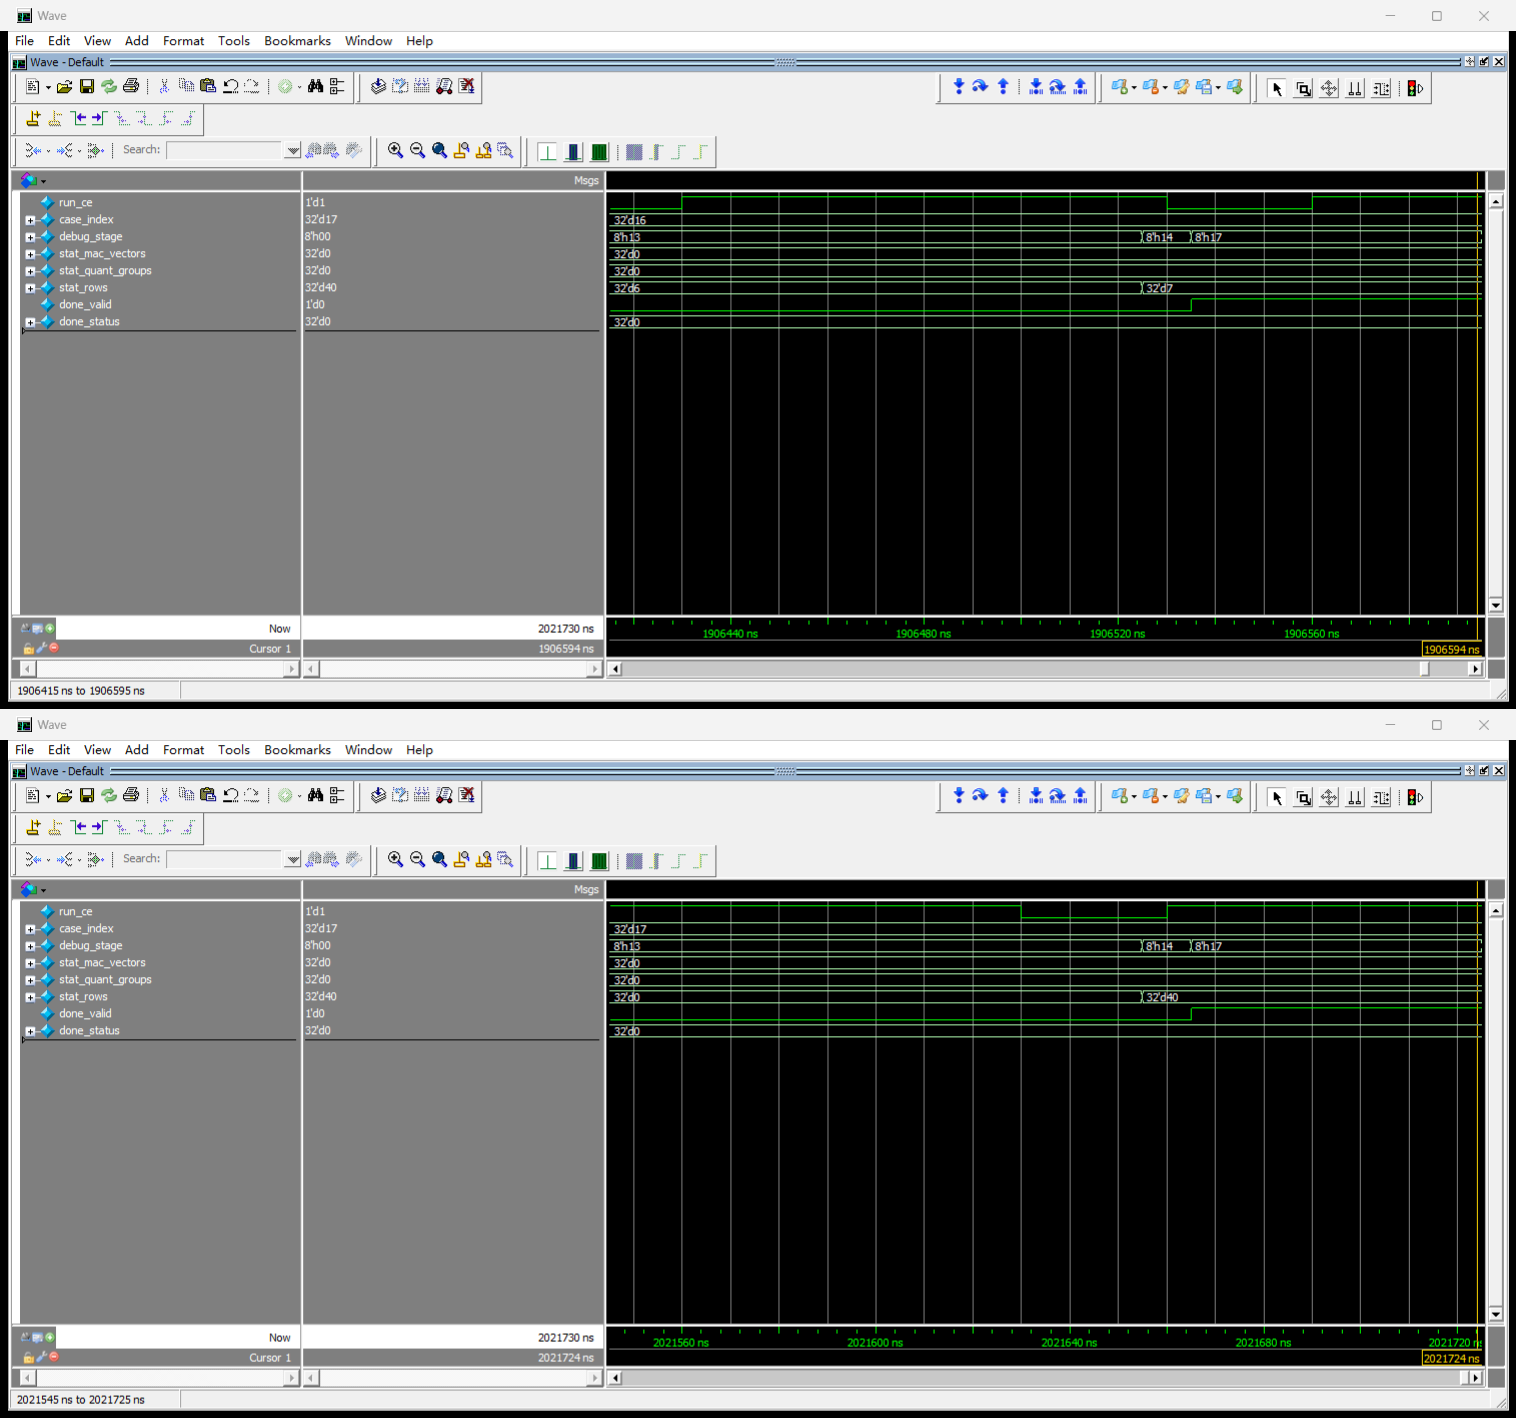
\includegraphics[width=\linewidth,height=0.52\textheight,keepaspectratio]{../figure/npu-simulation/pool-resize.png}
\caption{MaxPool与Resize的末行写回及完成波形}\label{fig:npu-pool-resize-validation}
\end{figure}

\FloatBarrier
